\documentclass[t]{beamer}

%\documentclass[handout, t]{beamer}
\setbeamertemplate{navigation symbols}{}
\usepackage{pstricks}
\usepackage{mathtools}
\usepackage{amsfonts}
\usepackage{mathrsfs}
\usepackage{amsmath}
\setbeamertemplate{navigation symbols}{}
\usepackage{bm}
\usepackage[UTF8]{ctex}
\usetheme{AnnArbor}
\usefonttheme{serif}
\useinnertheme{rounded}
%\usecolortheme{crane}
\setbeamertemplate{blocks}[rounded][shadow=true]
\usepackage{nicematrix}
\newcommand{\dif}{{\;\rm d}}
\usepackage{graphicx}
\usepackage{pgf}
\usepackage{tikz}
\usetikzlibrary{arrows, decorations.pathmorphing, backgrounds, positioning, fit, petri, automata}
\tikzset{>=stealth}

\usepackage{setspace}
\setmainfont{Times New Roman}
\setCJKmainfont{Microsoft YaHei}


\hypersetup{pdfpagemode=FullScreen}
\renewcommand{\Pr}{\mathbb{P}}
\usepackage{blkarray}


\setbeamercolor{block title}{bg=red!10!white}
\setbeamercolor{block body}{bg=gray!10!white}

\usepackage{multicol}
\newcommand{\E}{\mathbb{E}}
\newcommand{\EP}{\mathbb{E}^{\mathbb{P}}}
\newcommand{\EQ}{\mathbb{E}^{\mathbb{Q}}}
\newcommand{\Var}{{\rm Var}}
\newcommand{\Cov}{{\rm Cov}}


\begin{document}
\fontsize{11}{18}\selectfont


\CTEXindent



  \title{第二章~~离散时间马氏链2}
\author{应用随机过程}
\date{中国人民大学出版社}
  \begin{frame}
    \maketitle
  \end{frame}

\begin{frame}{本章内容}
    \begin{multicols}{2}
    \tableofcontents
    \end{multicols}
\end{frame}


\section{平稳分布}
\begin{frame}{平稳分布}
    一个非周期性,且有限状态的不可约马氏链收敛于一个平稳分布$\{\pi(y),\; y\in S\}$,即:
    \[\lim_{n\to\infty}p^n(x,y)= \pi(y) \]

    运用条件概率的定义:
\[\begin{split}
\Pr(X_n=j)&=\sum_i \Pr(X_0=i,X_n=j)\\
&=\sum_i \Pr(X_0=i)\Pr(X_n=j\;|\;X_0=i)
=\sum_i q(i) p^n(i,j)
\end{split} \]
其中,$q(i)=\Pr(X_0=i)$是初始概率。
\end{frame}


\begin{frame}{$\Pr(X_n=j)=\sum_i q(i) p^n(i,j)$的矩阵-向量形式}
    由$q(i),\;i\in S$组成的概率向量$\bf q$构成初始概率分布,并将之右乘转移概率矩阵${\bf P}^n$,可得$n$期概率所组成的向量${\bf q}_n$,具体如下:
    \[\begin{split}
    {\bf q}{\bf P}^n&=\underbrace{\begin{bmatrix}
    q(1)&q(2)&\cdots&q(k)
    \end{bmatrix}}_{\text{初始概率向量}}
    \overbrace{\begin{bmatrix}
    p^n(1,1) & p^n(1,2)&\cdots & p^n(1,k)\\
    p^n(2,1) &p^n(2,2)&\cdots & p^n(2,k)\\
    \vdots&\vdots&\ddots&\vdots\\
    p^n(k,1) &p^n(k,2)&\cdots & p^n(k,k)\\
    \end{bmatrix}}^{\text{$n$阶转移概率矩阵}}\\
    &=\begin{bmatrix}
    \sum\limits_{i=1}^k q(i)p^n(i,1)&\sum\limits_{i=1}^k q(i)p^n(i,2)&\cdots&\sum\limits_{i=1}^k q(i)p^n(i,k)
    \end{bmatrix}\\
    &=\begin{bmatrix}
    \Pr(X_n=1)&\Pr(X_n=2)&\cdots&\Pr(X_n=k)
    \end{bmatrix}\\
    &={\bf q}_n
    \end{split} \]

\end{frame}


\begin{frame}{$n$期概率分布的矩阵-向量形式}
\[\Pr(X_n=j)=\sum_i q(i)p^n(i,j)\quad\Rightarrow\quad{\bf q}{\bf P}^n={\bf q}_n\]
    在已知初始概率分布${\bf q}$的基础上,对其乘以$n$阶转移概率矩阵${\bf P}^n$,最终可得$n$期概率分布${\bf q}_n$。
\end{frame}

\subsection{平稳概率分布}
\begin{frame}{平稳概率分布和极限分布}
    记${\bf q}{\bf P}^n=\bm{\pi}$,如果$\bm{\pi}{\bf P}=\bm{\pi}$,则称$\bm{\pi}$为{平稳概率向量},其中的各元素组成{平稳概率分布};如果$\lim\limits_{n\to\infty}\Pr(X_n=i)=\bar\pi(i)$,此时称$\bar\pi(i)$组成的是{极限分布}。

    \begin{block}{说明:}
        对于不可约、非周期(irreducible \& aperiodic)的马氏链,其平稳分布和极限分布是{相等}的。  
    \end{block}
\end{frame}

\begin{frame}{社会流动问题中的平稳概率分布}
    假设$X_n$是一个家族第$n$代所处社会阶层的情况。假设总共有三个阶层,阶层间的代际转移概率矩阵如下所示:
    \begin{center}
        \begin{blockarray}{cccc}
            & 1&2&3\\
            \begin{block}{c[ccc]}
               1&0.7   &   0.2           & 0.1\\
               2&	0.3     &      0.5   &   0.2 \\
               3&	0.2   &   0.4 &          0.4 \\
               \end{block}		
        \end{blockarray}
    \end{center}
    求平稳状态下,该家族处于三个社会阶层的概率分别是多少?
\end{frame}

\begin{frame}{社会流动问题中的平稳概率分布(cont.)}
    由题意,可知:
    \[{\bf P}=	
            \begin{bmatrix}
    0.7   &   0.2           & 0.1\\
        0.3     &      0.5   &   0.2 \\
        0.2   &   0.4 &          0.4 \\
            \end{bmatrix} 
    \]
    方程$\bm{\pi}{\bf P}=\bm{\pi}$可以表达为:
    \[\begin{bmatrix}
    \pi_1&\pi_2&\pi_3
    \end{bmatrix}\begin{bmatrix}
    0.7   &   0.2           & 0.1\\
    0.3     &      0.5   &   0.2 \\
    0.2   &   0.4 &          0.4 \\
    \end{bmatrix}=\begin{bmatrix}
    \pi_1&\pi_2&\pi_3
    \end{bmatrix} \]
\end{frame}

\begin{frame}{社会流动问题中的平稳概率分布(cont.)}
    求解平稳概率分布就转化为对上式中的$\pi_1, \pi_2, \pi_3$进行求解,可得:
    \[\begin{cases}
    0.7\pi_1+0.3\pi_2+0.2\pi_3=\pi_1\\
    0.2\pi_1+0.5\pi_2+0.4\pi_3=\pi_2\\
    0.1\pi_1+0.2\pi_2+0.4\pi_3=\pi_3 \\
    \pi_1+\pi_2+\pi_3=1\\
    \end{cases} \]
    最终可得:$$\pi_1=\frac{22}{47},\qquad \pi_2=\frac{16}{47},\qquad \pi_3=\frac{9}{47}$$
    需要说明的是,上面的方程组在进行计算时,除最后一个作为概率完备性的约束条件必须保留外,其余的三个方程应当删去一个多余的。
\end{frame}


\begin{frame}{使用软件求解的基本思路}
    \small  \[\begin{cases}
        0.7\pi_1+0.3\pi_2+0.2\pi_3=\pi_1\\
        0.2\pi_1+0.5\pi_2+0.4\pi_3=\pi_2\\
        0.1\pi_1+0.2\pi_2+0.4\pi_3=\pi_3\\
        \pi_1+\pi_2+\pi_3=1\\
        \end{cases}\Rightarrow \quad \begin{cases}
        -0.3\pi_1+0.3\pi_2+0.2\pi_3=0\\
        0.2\pi_1-0.5\pi_2+0.4\pi_3=0\\
        \pi_1+\pi_2+\pi_3=1\\
        \end{cases}\]
        上面的方程组可化为如下矩阵形式:
        \[\underbrace{\begin{bmatrix}
        \pi_1&\pi_2&\pi_3
        \end{bmatrix}}_{\bm\pi}\underbrace{\begin{bmatrix}
        -0.3& 0.2& 1\\
        0.3 &-0.5&1\\
        0.2& 0.4& 1
        \end{bmatrix}}_{\bf A}=\underbrace{\begin{bmatrix}
        0&0&1
        \end{bmatrix}}_{\bf b} \]
        从而得到:
        \[\bm{\pi}{\bf A}={\bf b}\quad \Rightarrow\quad \bm{\pi}={\bf b}{\bf A}^{-1} \]
    \end{frame}


    \begin{frame}{使用软件求解的基本思路(cont.)}
        \small
        
        
        \[\bm{\pi}={\bf b}{\bf A}^{-1}=\begin{bmatrix}
        0&0&1
        \end{bmatrix}\begin{bmatrix}
        -0.3& 0.2& 1\\
        0.3 &-0.5&1\\
        0.2& 0.4& 1
        \end{bmatrix}^{-1} \]
        其中:\[{\bf A}^{-1}=\begin{bmatrix}
        -0.3& 0.2& 1\\
        0.3 &-0.5&1\\
        0.2& 0.4& 1
        \end{bmatrix}^{-1}=\begin{bmatrix}
        -90/47& 20/47& 70/47\\
        -10/47& -50/47& 60/47\\
        22/47& 16/47& 9/47
        \end{bmatrix}\]
        可见,$\bm{\pi}$的结果,刚好就是对应的${\bf A}^{-1}$的最后一行,即:
        \[\bm{\pi}=\begin{bmatrix}
            \displaystyle\frac{22}{47} &\displaystyle\frac{16}{47}&\displaystyle\frac{9}{47}
        \end{bmatrix} \]
\end{frame}


\begin{frame}{使用软件求解的注意事项}
    \begin{spacing}{1.2}
        \small
        $\bm{\pi}={\bf b}{\bf A}^{-1}$使用的前提是矩阵${\bf A}$可逆(invertible)。
    
        以赌徒破产问题为例,相应的转移概率矩阵${\bf P}$与求解用到的${\bf A}$分别如下:
        \[{\bf P}=\begin{bmatrix}
         1 & 0 & 0 & 0 & 0 & 0\\
         0.6 & 0 & 0.4 & 0 & 0 & 0\\
         0 & 0.6 & 0 & 0.4 & 0 & 0\\
         0 & 0 & 0.6 & 0 & 0.4 & 0\\
         0 & 0 & 0 & 0.6 & 0 & 0.4\\
         0 & 0 & 0 & 0 & 0 & 1\\
        \end{bmatrix},\quad 
        {\bf A}=\begin{bmatrix}
            0 &   0 &   0 &   0 &   0  &  1\\
            0.6&   -1  &  0.4 &   0 &   0  &  1\\
            0  &  0.6  & -1 &   0.4 &   0  &  1\\
           0 &   0  &  0.6 &  -1  &  0.4 &   1\\
            0 &   0 &   0 &   0.6 &  -1 &   1\\
            0 &   0 &   0 &   0 &   0 &   1\\
        \end{bmatrix} \]
        这里的矩阵${\bf A}$不是满秩的(该矩阵的秩为5),因此不存在逆矩阵。
    \end{spacing}

\end{frame}


\begin{frame}{遍历马氏链}
    对于非周期、不可约且状态有限的马氏链,可以利用$\bm{\pi}={\bf b}{\bf A}^{-1}$正常计算平稳概率分布。
    
    由于这类马氏链具有良好的性质,因此也称为遍历马氏链(ergodic Markov chain)。之所以称其为“遍历马氏链”,是因为这类马氏链的各状态均是常返的,在有限时间内可以访问状态空间中的各个状态。
\end{frame}

\subsection{双随机链}
\begin{frame}{双随机链}
    若马氏链的转移概率矩阵各列元素之和均为1,则称其是双随机链(doubly stochastic chain),即:
    \[\sum_x p(x,y)=1\]
    
    在双随机链当中,其各行和各列的元素之和均等于1,即:
\[\sum_x p(x,y)=1,\qquad \text{同时}\qquad \sum_y p(x,y)=1 \]


\end{frame}

\begin{frame}{双随机链的性质}
    若$\bf P$是$N$个状态马氏链的双随机转移概率,则均匀分布$\pi(x)=1/N,\;\forall x$是其平稳分布。

    \begin{block}{推论:}
        若$\bf P$是$N$个状态马氏链的转移概率,且均匀分布$\displaystyle\pi(x)=\frac{1}{N},\;\forall x$是其平稳分布,则$\bf P$是双随机的。
    \end{block}
\end{frame}

\subsection{细致平衡条件}
\begin{frame}{细致平衡条件}
    如果$\pi(x)p(x,y)=\pi(y)p(y,x)$,则称$\bm{\pi}$满足细致平衡条件(detailed balance condition)。

    原先的$\bm{\pi}{\bf P}=\bm{\pi}$说明,在所有的转移结束后,每个状态的概率与初始时的概率相等,即:
\begin{equation*}
\begin{split}
{\sum_x \pi(x)p(x,y)}&=\pi(y)={\pi(y)\sum_{x}p(y,x)} \\
&=\sum_{x}\pi(y)p(y,x)
\end{split}
\end{equation*}
而在细致平衡条件下,从状态$x${一步}转移到状态$y$的概率,刚好等于从状态$y${一步}转移到状态$x$的概率,即:
\begin{equation*}
\pi(x)p(x,y)=\pi(y)p(y,x)
\end{equation*}
\end{frame}



\begin{frame}{细致平衡条件(cont.)}
\[\sum_x \pi(x)p(x,y)=\sum_{x}\pi(y)p(y,x) \]
\[\pi(x)p(x,y) = \pi(y)p(y,x) \]

上面两个等式之间唯一的区别就是一个求和符号。但是可以看出:细致平衡条件比之前的$\bm{\pi}{\bf P}=\bm{\pi}$更严格,因为其要求对应的项必须严格相等。正因为如此,满足细致平衡条件的马氏链一定存在平稳分布;但是具有平稳分布的马氏链不一定满足细致平衡条件。

细致平衡条件可以降低平稳分布在计算上的难度,并且该条件经常被运用于可数状态马氏链的平稳分布求解问题中。
\end{frame}


\begin{frame}{举例9:生灭链}
    假设某物种在下个阶段可能会发生如下变化:产生一个新个体的概率为0.3;死亡的概率为0.2;未发生任何变化的概率为0.5。对于7期的马氏链,最终的转移概率矩阵如下:
    \[\begin{bmatrix}
    0.7 & 0.3 & 0 & 0 & 0 & 0 & 0\\ 
    0.2 & 0.5 & 0.3 & 0 & 0 & 0 & 0\\ 
    0 & 0.2 & 0.5 & 0.3 & 0 & 0 & 0\\ 
    0 & 0 & 0.2 & 0.5 & 0.3 & 0 & 0\\ 
    0 & 0 & 0 & 0.2 & 0.5 & 0.3 & 0\\ 
    0 & 0 & 0 & 0 & 0.2 & 0.5 & 0.3\\ 
    0 & 0 & 0 & 0 & 0 & 0.2 & 0.8\\ 
    \end{bmatrix} \]
    求其平稳分布。
\end{frame}


\begin{frame}{生灭链(cont.)}
    \begin{spacing}{1}
      \small
    经过验证可以发现,该链并不违反细致平衡条件。根据细致平衡条件,可以列出如下等式:
    \[\pi(i)p(i,i+1)=\pi(i+1)p(i+1,i),\qquad i=1,2,\ldots,6 \]
    即:$$0.3\pi(i)=0.2\pi(i+1)\;\Rightarrow\; \pi(i+1)=1.5\pi(i), \quad i=1,2,\ldots,6$$
    
    利用$\displaystyle\sum_{i=1}^7 \pi(i)=1$,并假设$\pi(1)=c$,最终可得:
    \[c\left(1+1.5+1.5^2+\cdots+1.5^6\right)=1\quad \Rightarrow\quad c=\frac{1.5-1}{1.5^7-1}\approx 0.0311 \]
    于是:$$\bm{\pi}=\begin{bmatrix}
    0.0311& 0.0466& 0.0699& 0.1049& 0.1574& 0.2360& 0.3541 
    \end{bmatrix}$$  
    \end{spacing}
\end{frame}


\begin{frame}{举例10:图上的随机游走}
    假设有一个包含五个顶点的图,每个顶点会以等概率游走至相邻的顶点。
\begin{center}
            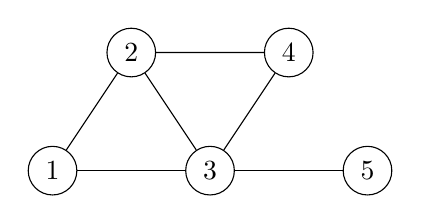
\begin{tikzpicture}
            \node[draw,circle] (A) at (0,0) {1};
            \node[draw,circle] (B) at (1,1.5) {2};
            \node[draw,circle] (C) at (2,0){3};
            \node[draw,circle] (D) at (3,1.5){4};
            \node[draw,circle] (E) at (4,0){5};
            
            \draw(A)--(B)--(D)--(C);
            \draw(A)--(C)--(E);
            \draw(B)--(C);
    \end{tikzpicture}
        \end{center}
    求由此构成的马氏链的平稳分布。
        
\end{frame}

\begin{frame}{图上的随机游走(cont.)}
    该问题当中,相邻两个顶点之间的转移概率均为正,因此不违反细致平衡条件。
    首先构造对应的转移概率矩阵$\bf P$:
    \[{\bf P}=	
            \begin{bmatrix}
    \vspace{1ex}0  &      \dfrac{1}{2} &       \dfrac{1}{2} &        0&        0  \\
    \vspace{1ex}
    \dfrac{1}{3}  &       0 &        \dfrac{1}{3} &      \dfrac{1}{3}&        0  \\
    \vspace{1ex}\dfrac{1}{4}  &     \dfrac{1}{4} &        0 &        \dfrac{1}{4} &       \dfrac{1}{4}   \\
    \vspace{1ex}0  &     \dfrac{1}{2}  &       \dfrac{1}{2}  &        0 &        0 \\
    0  &       0 &       1 &        0 &        0 \\
            \end{bmatrix}\]
        \end{frame}
        
        \begin{frame}{图上的随机游走(cont.)}
            \small
    根据细致平衡条件,可列出如下方程组:
    \[\begin{cases}
    \pi(1)p(1,2)=\pi(2)p(2,1)\\
    \pi(1)p(1,3)=\pi(3)p(3,1)\\
    \pi(4)p(4,2)=\pi(2)p(2,4)\\
    \pi(4)p(4,3)=\pi(3)p(3,4)\\
    
    \pi(5)p(5,3)=\pi(3)p(3,5)\\
    \end{cases}\Rightarrow\quad  \begin{cases}
     \vspace{1ex} \dfrac{1}{2}\pi(1)=\dfrac{1}{3}\pi(2)\\  \vspace{1ex} 
    \dfrac{1}{2}\pi(1)=\dfrac{1}{4}\pi(3)\\  \vspace{1ex} 
    \dfrac{1}{2}\pi(4)=\dfrac{1}{3}\pi(2)\\  \vspace{1ex} 
    \dfrac{1}{2}\pi(4)=\dfrac{1}{4}\pi(3)\\ 
    \pi(5)=\dfrac{1}{4}\pi(3)\\
    \end{cases}\]
    令$\pi(3)=c$,可得:
    \[\pi(1)=\dfrac{1}{2}c,\quad \pi(2)=\dfrac{3}{4}c,\quad \pi(4)=\dfrac{1}{2}c,\quad \pi(5)=\dfrac{1}{4}c\]       \end{frame}
        
    \begin{frame}{图上的随机游走(cont.)}
        \small
    由于$\displaystyle\sum_i \pi(i)=1$,因此:$$c=\frac{1}{3}$$
    最终可得:
    \[\pi(1)=\frac{2}{12},\quad \pi(2)=\frac{3}{12},\quad \pi(3)=\frac{4}{12},\quad \pi(4)=\frac{2}{12},\quad \pi(5)=\frac{1}{12}\]
\begin{center}
    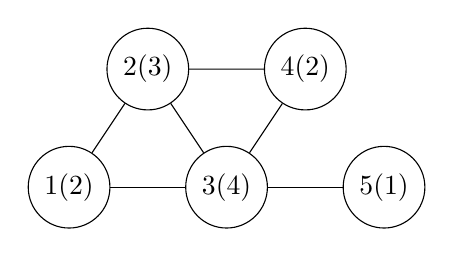
\begin{tikzpicture}
        \node[draw,circle] (A) at (0,0) {1(2)};
        \node[draw,circle] (B) at (1,1.5) {2(3)};
        \node[draw,circle] (C) at (2,0){3(4)};
        \node[draw,circle] (D) at (3,1.5){4(2)};
        \node[draw,circle] (E) at (4,0){5(1)};
        
        \draw(A)--(B)--(D)--(C);
        \draw(A)--(C)--(E);
        \draw(B)--(C);
        \end{tikzpicture}
\end{center}
\end{frame}

\subsection{马氏链的可逆性}
\begin{frame}{马氏链的可逆性(reversible)}
    $\{X_0,X_1,\ldots,X_n\}$是从平稳分布$\pi(i)$开始的遍历马氏链,若逆向观察$X_m$, $0\le m\le n$,则$\{X_n,X_{n-1}, \ldots,X_0\}$也构成一个马氏链。
\begin{center}
    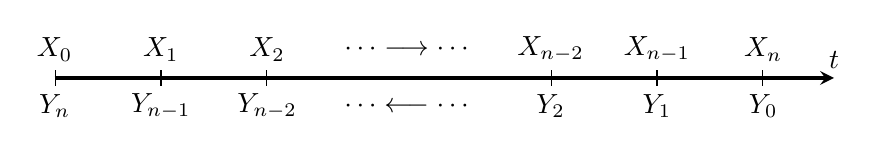
\begin{tikzpicture}[>=stealth,scale=.9]
        \draw [->, very thick] (0,0)--(11,0);
        \draw [|-|](0,0)--(1.5,0);
        \draw [|-|](3,0)--(1.5,0);
        \draw [|-|](7,0)--(8.5,0);
        \draw [|-|](8.5,0)--(10,0);
        
        \node at (10,.4) {$X_n$};
        \node at (8.5,.4) {$X_{n-1}$};
        \node at (7,.4) {$X_{n-2}$};
        \node at (0,.4) {$X_0$};
        \node at (1.5,.4) {$X_1$};
        \node at (3,.4) {$X_2$};
        \node at (5,.4) {$\cdots\longrightarrow \cdots$};
        
        \node at (11,.25) {$t$};
        
        
        \node at (10,-.4) {$Y_0$};
        \node at (8.5,-.4) {$Y_1$};
        \node at (7,-.4) {$Y_2$};
        \node at (0,-.4) {$Y_n$};
        \node at (1.5,-.4) {$Y_{n-1}$};
        \node at (3,-.4) {$Y_{n-2}$};
        \node at (5,-.4) {$\cdots\longleftarrow\cdots$};
        
        \end{tikzpicture}
\end{center}

基于$\{X_0,X_1,\ldots,X_n,\ldots X_{n+k}\}$构成的马氏链的可逆性可得:
\begin{align*}
\Pr(X_{n+1}|X_n,X_{n-1}\ldots X_0)&=\Pr(X_{n+1}|X_n)\\
\Pr(X_{n-1}|X_n,X_{n+1}\ldots X_{n+k})&=\Pr(X_{n-1}|X_n)
\end{align*}

\end{frame}


\begin{frame}{马氏链的可逆性(cont.)}
    根据贝叶斯定理可得:
    \[\Pr(X_{n-1}|X_n)=\frac{\Pr(X_{n}|X_{n-1})\Pr(X_{n-1})}{\Pr(X_n)} \]
    注意到,$\Pr(X_n)$的取值会因$n$的不同而有所变化,因此$\Pr(X_{n-1}|X_n)$的取值也会受到$n$的影响。正因如此,
    原马氏链的反向链$\{X_n,X_{n-1}, \ldots,X_0\}$不一定会满足时齐性。
    
    \begin{block}{注意:}
        马氏链的可逆性适用于遍历马氏链。对于具有吸收态的马氏链而言,可逆性显然不成立。  
    \end{block}

\end{frame}


\begin{frame}{对偶转移概率}
    对于遍历马氏链$\{X_0,X_1,\ldots,X_n\}$而言,若固定$n$且令$Y_m=X_{n-m},  0\le m\le n$,则$Y_m$是一个马氏链,其转移概率为\[\hat p(i,j)=\Pr(Y_{m+1}=j|Y_m=i)=\frac{\pi(j)p(j,i)}{\pi(i)} \]
    其中,$\hat p(i,j)$称为对偶(dual)转移概率。
\end{frame}


\begin{frame}{细致平衡条件与可逆性}
    当$\bm{\pi}$满足{细致平衡条件} $\pi(i)p(i,j)=\pi(j)p(j,i)$时,
    \[{\hat p(i,j)}=\frac{\pi(j)p(j,i)}{\pi(i)}=\frac{\pi(i)p(i,j)}{\pi(i)}={p(i,j)} \]
    即,在细致平衡条件下,逆向链的转移概率与原链相同。
\end{frame}


\begin{frame}{细致平衡条件与可逆性(cont.)}
    假设马氏链从$\pi$开始,分别经过状态$x_0,x_1,\ldots, x_n$,则:
    \[\begin{split}
    \Pr_{\pi}&\left({X_0=x_0,X_1=x_1,X_2=x_2,\ldots,X_n=x_n}\right)\\ &={\pi(x_0)p(x_0,x_1)}p(x_1,x_2)\cdots p(x_{n-1},x_n)\\
    &={{\pi(x_1)}{p(x_1,x_0)}}p(x_1,x_2)\cdots p(x_{n-1},x_n)\\
    &={\pi(x_2)}p(x_1,x_0){p(x_2,x_1)}\cdots p(x_{n-1},x_n)\\
     &=\cdots\cdots\\
    &=\pi(x_n)p(x_{n},x_{n-1})p(x_{n-1},x_{n-2})\cdots p(x_2,x_1)p(x_1,x_0)\\
    &=\Pr_{\pi}\left({\hat X_0=x_n,\hat X_1=x_{n-1},\ldots,\hat X_{n-1}=x_1, \hat X_n=x_0}\right)\\
    \end{split}\]
\end{frame}


\section{极限行为}
\begin{frame}{极限行为}
    如果$y$是一个非常返态,则对$\forall x$,均有:
    \[\sum_{n=1}^{\infty}p^n(x,y)<\infty \]
    从而
    $$\lim_{n\to\infty}p^n(x,y)= 0$$
    这意味着我们在考虑马氏链的极限行为时,只需将注意力集中在常返态上,
    特别是只包含一个不可约常返类的马氏链。
\end{frame}




\begin{frame}{相关定理}
    \begin{block}{收敛定理}
        假设${\bf P}$不可约、非周期且具有平稳分布$\bm{\pi}$,则:
        \begin{equation*}
        \lim_{n\to\infty}p^n(x,y)= \pi(y)
        \end{equation*}
    \end{block}
    
    \begin{block}{渐近频率定理}
        假设${\bf P}$不可约,且所有状态均是常返态,记$N_t(y)$为在时刻$t$之前访问$y$的总次数,则:
        \begin{equation*}
        \frac{N_t(y)}{t}\to \frac{1}{\E_y(\tau_y)},\qquad {\rm a.s.} 
        \end{equation*}
    \end{block}
\end{frame}


\begin{frame}{渐近频率定理的证明}
    证明需要使用大数定律。假设从时刻0到$t$,返回状态$y$的次数为$k$,记每次返回的时刻分别为$t_0, t_1,t_2,\ldots,t_k$ (其中$t_0=0,\; t_k=t$),每次返回的时间间隔分别为$\tau_1,\tau_2,\ldots,\tau_k$,则:
    \[\tau_i=t_i-t_{i-1},\qquad 1\le i\le k \]
   \begin{center}
    \begin{tikzpicture}[>=stealth, very thick,scale=.9]
        \draw [->](0,0)--(10,0);
        \foreach \x in {0,1.5,3,4.5, 8,9.5}
        {\draw (\x, -.1)--(\x, .1);
        \node at (\x, -1.25) {$y$};
        }
        \node at (0,-.5){$t_0=0$};
        \node at (1.5,-.5){$t_1$};
        \node at (3,-.5){$t_2$};
        \node at (4.5,-.5){$t_3$};
        \node at (8,-.5){$t_{k-1}$};
        \node at (9.5,-.5){$t_k=t$};
        
        \draw[|<->|] (0,.5)  to node[auto] {$\tau_1$} (1.5,.5);
        \draw[|<->|] (1.5,.5)  to node[auto] {$\tau_2$} (3,.5);
        \draw[|<->|] (3,.5)  to node[auto] {$\tau_3$} (4.5,.5);
        \draw[|<->|] (8,.5)  to node[auto] {$\tau_k$} (9.5,.5);
        
        \foreach \x in {.5,-.5,-1.25, -2}
        \node at (6.25,\x) {$\cdots$};
        
        \node at (-1.5,.5) {时间间隔};
        \node at (-1.5,-.5) {返回时间};
        \node at (-1.5,-1.25) {状态};
        \node at (-1.5,-2) {返回次数};
        
        
        \node at (0, -2) {$0$};
        \node at (1.5, -2) {$1$};
        \node at (3, -2) {$2$};
        \node at (4.5, -2) {$3$};
        
        \node at (8, -2) {$k-1$};
        \node at (9.5, -2) {$k$};
        
        \end{tikzpicture}
        
   \end{center}
\end{frame}


\begin{frame}{渐近频率定理的证明(cont.)}
    由大数定律可知:每次访问的时间间隔$\tau_i$是独立同分布的,因此,当$n\to\infty$时,可得:
    \[ \frac{\tau_1+\tau_2+\cdots+\tau_k}{k}= \frac{t}{k}\to \E_y(\tau_y),\qquad \text{a.s.}\]
    其中,$\E_y(\tau_y)$是从状态$y$首次返回的期望时间。
    这里的访问次数$k$就是$N_t(y)$,因此:
    \[\frac{N_t(y)}{t}\to \frac{1}{\E_y(\tau_y)},\qquad {\rm a.s.} \]
\end{frame}

\begin{frame}{定理}
    假设${\bf P}$不可约, 且具有平稳分布$\bm{\pi}$,则:
    \begin{equation*}
    \pi(y)=\frac{1}{\E_y(\tau_y)}
    \end{equation*}

    该定理说明:状态$y$下的平稳分布对应的概率$\pi(y)$等于首次返回状态$y$期望步数的倒数;并且在状态期间$n\to \infty$时等于返回状态$y$的次数占整个状态步数$n$的比例。
\end{frame}



\begin{frame}{简要证明}
    由于平稳分布$\bm{\pi}$满足:
\[\lim_{n\to\infty}p^n(x,y)=\pi(y),\qquad \forall x\in S \]
因此,相应的$\pi(y)$可以看作在转移步数$n\to \infty$时,到达状态$y$的“可能性”。故$\pi(y)$可以看成访问状态$y$的步数$N_n(y)$占总的转移步数$n$的“比重”,从而可得:
\begin{equation*}
\lim_{n\to\infty}\frac{N_n(y)}{n}=\pi(y)
\end{equation*}
根据前面的渐近频率定理可得:
\begin{equation*}
\E_y(\tau_y)=\frac{1}{\pi(y)} 
\end{equation*}
\end{frame}


\begin{frame}{回顾修复链}
    在修复链当中,状态空间$\{0,1,2,3,12,13,23\}$对应平稳分布的概率分别如下:
    \[\pi(0)=\frac{3000}{8910},\quad \pi(1)=\frac{500}{8910},\quad \pi(2)=\frac{1200}{8910},\quad \pi(3)=\frac{4000}{8910},\]
    \[\pi(12)=\frac{22}{8910},\quad \pi(13)=\frac{60}{8910},\quad \pi(23)=\frac{128}{8910} \]
    问:若让机器正常运转1800天,分别需要多少个零件1、零件2和零件3?
\end{frame}



\begin{frame}{修复链(cont.)}\small
    各零件需替换的概率分别为:
    \[\begin{split}
    \text{零件1:}&\quad \pi(12)+\pi(13)=\frac{22}{8910}+\frac{60}{8910}=\frac{82}{8910}\\
    \text{零件2:}&\quad \pi(12)+\pi(23)=\frac{22}{8910}+\frac{128}{8910}=\frac{150}{8910}\\
    \text{零件3:}&\quad \pi(13)+\pi(23)=\frac{60}{8910}+\frac{128}{8910}=\frac{188}{8910}\\
    \end{split}\]
    根据$\displaystyle\lim_{n\to\infty}\frac{N_n(y)}{n}=\pi(y)$的变形形式:
    \[N_n(y)\to n\cdot \pi(y),\qquad \text{a.s.}\]
    可以得到需要的各零件的数量如下:
    \[
    \text{零件1:}\quad 1800\times \frac{82}{8910} =16.56(\text{个})\qquad
    \text{零件2:}\quad 1800\times\frac{150}{8910} =30.3(\text{个})\]\[
    \text{零件3:}\quad 1800\times\frac{188}{8910} =37.98(\text{个})
    \]
\end{frame}


\begin{frame}{库存链}
    假设每销售一单位的商品,可获得12元的利润,但在店里存储一单位商品的花费为2元/天。商品每天的需求量$k$不超过3单位。
    \begin{center}
    \begin{tabular}{c|cccc}
    \hline
    $k$ &0 &1& 2& 3\\
    \hline
    $\Pr$&0.3&0.4&0.2&0.1\\
    \hline
    \end{tabular}
    \end{center}
    
    问:在以下三种策略下,每天净利润的期望值分别是多少?

    \begin{enumerate}
        \item $s=2$, $S=3$库存策略;
        \item  $s=1$, $S=3$库存策略;
        \item  $s=0$, $S=3$库存策略。
        \end{enumerate}
        其中,$s$表示需要补货的最大库存(即前一天库存若达到该值或以下,就需要在第二天之前补足库存);$S$表示库存的最大数量。
\end{frame}

\begin{frame}{$s=2$, $S=3$库存策略}
\begin{center}
    \begin{blockarray}{ccccc}
        & 0 & 1 &2	&3  \\	
            \begin{block}{c[cccc]}
    0& 0.1  &       0.2 &        0.4 &        0.3  \\
    1 &0.1  &       0.2 &        0.4 &        0.3  \\
    2 &0.1  &       0.2 &        0.4 &        0.3  \\
    3&0.1  &       0.2 &        0.4 &        0.3  \\
            \end{block} 
    \end{blockarray}
\end{center}
平稳概率分布如下:
\[\pi(0)=0.1, \quad \pi(1)=0.2, \quad \pi(2)=0.4,\quad\pi(3)=0.3 \]
\end{frame}

\begin{frame}{$s=2$, $S=3$库存策略(cont.)}
    根据商品需求量对应的表格,销售额为:
\[12\times (0.3\times 0+0.4\times 1+0.2\times 2+0.1\times 3)=13.2\text{(元/天)} \]
库存的花费为:
\[2\times (0.1\times 0+0.2\times 1+0.4\times 2+0.3\times 3)=3.8\text{(元/天)}\]
每天净利润的期望值为:
$$13.2-3.8=9.4\text{(元)}$$
\end{frame}



\begin{frame}{$s=1$, $S=3$库存策略}
\begin{center}
    \begin{blockarray}{ccccc}
        & 0 & 1 &2	&3  \\	
            \begin{block}{c[cccc]}
    0& 0.1  &       0.2 &        0.4 &        0.3  \\
    1 &0.1  &       0.2 &        0.4 &        0.3  \\
    2 &0.3  &       0.4 &        0.3 &        0  \\
    3&0.1  &       0.2 &        0.4 &        0.3  \\
            \end{block} 
    \end{blockarray}
\end{center}
平稳概率分布如下:
\[\pi(0)=\frac{19}{110}, \quad \pi(1)=\frac{30}{110}, \quad \pi(2)=\frac{40}{110},\quad\pi(3)=\frac{21}{110} \]
\end{frame}



\begin{frame}{$s=1$, $S=3$库存策略(cont.)}
注意,当存货为2时,若需求量为3,则只能售出2件商品,因此
该策略下的销售额应当扣减这一情形。
该事件的概率为:$$\pi(2)\times\Pr(k=3)=\frac{40}{110}\times 0.1=0.036$$
相应的销售额为:
\[13.2-0.036\times 12=12.764\text{(元/天)}
\]
库存的花费为:
\[2\times \left(\frac{19}{110}\times 0+\frac{30}{110}\times 1+\frac{40}{110}\times 2+\frac{21}{110}\times 3\right)=3.145\text{(元/天)}\]
每天净利润的期望值为:
$$12.764-3.145=9.619\text{(元)}$$
\end{frame}



\begin{frame}{$s=0$, $S=3$库存策略}
\begin{center}
    \begin{blockarray}{ccccc}
        & 0 & 1 &2	&3  \\	
            \begin{block}{c[cccc]}
    0& 0.1  &       0.2 &        0.4 &        0.3  \\
    1 &0.7  &       0.3 &        0 &        0  \\
    2 &0.3  &       0.4 &        0.3 &        0  \\
    3&0.1  &       0.2 &        0.4 &        0.3  \\
            \end{block} 
    \end{blockarray}
\end{center}
平稳概率分布如下:
\[\pi(0)=\frac{343}{1070}, \quad \pi(1)=\frac{300}{1070}, \quad \pi(2)=\frac{280}{1070},\quad\pi(3)=\frac{147}{1070} \]
\end{frame}


\begin{frame}{$s=0$, $S=3$库存策略(cont.)}
\begin{center}
\begin{tabular}{c|cccc}
\hline
$k$ &0 &1& 2& 3\\
\hline
$\Pr$&0.3&0.4&0.2&0.1\\
\hline
\end{tabular}
\end{center}
注意,此时仍存在存货小于需求量的情形,此类事件的概率为:
\small
\[\begin{split}
\pi(2)\times\Pr(k=3)&\times(3-2) +\pi(1)\times \left[\Pr(k=3)\times(3-1)+\Pr(k=2)\times(2-1)\right]\\
&=\frac{280}{1070}\times 0.1\times 1+\frac{300}{1070}\times \left(0.1\times 2+0.2\times 1\right)\\
&=\frac{148}{1070}
\end{split}\]
\end{frame}



\begin{frame}{$s=0$, $S=3$库存策略(cont.)}
相应的销售额为:
\[13.2-\frac{148}{1070}\times 12=11.54\text{(元/天)}
\]
库存的花费为:
\[2\times \left(\frac{343}{1070}\times 0+\frac{300}{1070}\times 1+\frac{280}{1070}\times 2+\frac{147}{1070}\times 3\right)=2.43\text{(元/天)}\]
每天净利润的期望值为:
$$11.54-2.43=9.11\text{(元)}$$
\end{frame}



\section{离出分布和离出时间}

\subsection{离出分布}
\begin{frame}{离出分布的含义}
    离出分布(exit distribution)考查的是:对于至少存在两个不同吸收态的马氏链,从给定的非常返态$j$开始,该马氏链最终进入某一特定吸收态$i$的{概率}是多少?

    换句话说,离出分布考查的是一个非常返态$j$最终被某一状态$i$吸收的概率(即{吸收概率},absorption probability)。
    
    比如:在赌徒破产模型中,有两个吸收态(破产和赚钱离场),赌徒进入赌场,最终破产或赚钱离场的概率分别是多少?这里所要求得的概率就是吸收概率。在前面的式(2.5)中已经给出了吸收概率的最终取值。本节则是侧重于如何计算这些概率。
\end{frame}


\begin{frame}{离出分布的计算}
    记非常返态$x$最终被状态$z$吸收的概率为$h(x)=\Pr(X_{\tau}=z|X_0=x)$,根据C-K方程可得:
    \[\begin{split}
    \Pr(X_{\tau}=z|X_0=x)&=\sum_y \Pr(X_{\tau}=z|X_1=y){\Pr(X_1=y|X_0=x)}\\
    &=\sum_y \Pr(X_{\tau}=z|X_1=y)\cdot {p(x,y)}\\
    \end{split} \]
    因此:
    \begin{equation*}
    h(x)=\sum_y p(x,y)\cdot h(y)
    \end{equation*}
\end{frame}

\begin{frame}{举例11:两年制大学}
	在当地一所两年制大学里,60\%的新生可升到二年级,25\%仍为一年级学生,15\%退学;70\%的二年级学生毕业,20\%仍为二年级学生,10\%退学。
	
    问:新生最终毕业的比例是多少?
    
    \begin{block}{思路:}
        在此问题中,存在两个吸收态(常返态):“毕业”和“退学”。相应的问题就转化成:给定当前状态为“新生”,马氏链最终进入吸收态“毕业”的概率是多少?
    \end{block}
\end{frame}

\begin{frame}{两年制大学(cont.)}
状态空间\{1,2,G,D\}中的状态1、2、G、D分别表示一年级、二年级、毕业(graduate)和退学(dropout),得到相应的转移概率矩阵如下:
\begin{center}
\begin{blockarray}{ccccc}
		&1 & 2 & G &D  \\	
	\begin{block}{c[cccc]}
		1 &0.25 &      0.6&    0&    0.15 \\
		2 & 0   &      0.2&  0.7&    0.1\\
		G &  0  &        0&    1&    0      \\
		D &0    &       0 &   0 &        1 \\			
	\end{block}
\end{blockarray}
\end{center}
\end{frame}



\begin{frame}{两年制大学(cont.)}\small
    用$h(x)$表示现在状态是$x$的学生最终毕业的概率,可得:
    \[\begin{cases}
     \vspace{1ex}  h(1)=\displaystyle\sum_{s\in S} p(1,s)\cdot h(s)=p(1,1)h(1)+p(1,2)h(2)+p(1,G)h(G)+p(1,D)h(D)\\
    h(2)=\displaystyle\sum_{s\in S} p(2,s)\cdot h(s)=p(2,1)h(1)+p(2,2)h(2)+p(2,G)h(G)+p(2,D)h(D)
    \end{cases} \]
    
    由于$h(G)=1,\quad h(D)=0$,因此:
    \[\begin{cases}
    h(1)=0.25h(1)+0.6h(2)\\
    h(2)=0.2h(2)+0.7
    \end{cases} \quad\Rightarrow\quad \begin{cases}
    h(1)=0.7\\
    h(2)=0.875
    \end{cases}\]
    因此,新生最终毕业的概率是0.7;二年级学生最终毕业的概率是0.875。
\end{frame}


\begin{frame}{矩阵-向量的形式重新表述}
    \[\begin{bmatrix}
        h(1)\\
        h(2)\\
        \end{bmatrix}=\begin{bmatrix}
        0.25 & 0.6\\
        0 &0.2
        \end{bmatrix}\begin{bmatrix}
        h(1)\\h(2)
        \end{bmatrix}+\begin{bmatrix}
        0\\0.7
        \end{bmatrix} \]
        相应的矩阵形式如下:
        \begin{equation*}
        {\bf h}={\bf Ah}+{\bf b}
        \end{equation*}
        其中,${\bf h}$是由$h(1)$和$h(2)$组成的列向量;${\bf A}$是由非常返态1和2组成的分块矩阵;${\bf b}$是由吸收态G(毕业)与非常返态1和2组成的分块矩阵。
        对上式进行简单的运算,可得:
        \begin{equation*}
       {\bf h}=({\bf I}-{\bf A})^{-1}{\bf b}={\bf M}{\bf b}
       \end{equation*}
       其中,${\bf I}$是主对角线元素均为1的单位矩阵(identity matrix)。 ${\bf M}=({\bf I}-{\bf A})^{-1}$称作基础矩阵(fundamental matrix)   
\end{frame}

\begin{frame}{转移概率矩阵分块}
    \[\left[\begin{array}{cc|c|c}
        0.25 &      0.6&    0&    0.15 \\
         0   &      0.2&  0.7&    0.1\\\hline
        0  &        0&    1&    0      \\
        0    &       0 &   0 &        1 \\
        \end{array}\right] \]
        其中:\[{{\bf A}=\begin{bmatrix}
            0.25&0.6\\0&0.2
            \end{bmatrix}},\qquad {{\bf b}=\begin{bmatrix}
            0\\0.7
            \end{bmatrix}}\]
\end{frame}

\begin{frame}{回顾赌徒破产问题}
    转移概率矩阵如下:
    \begin{center}
    \begin{blockarray}{ccccccc}
        & 0&1&2&3&4&5\\
        \begin{block}{c[cccccc]}
            0&1 & 0 & 0 & 0 & 0 & 0\\
    1&0.6 & 0 & 0.4 & 0 & 0 & 0\\
    2&0 & 0.6 & 0 & 0.4 & 0 & 0\\
    3&0 & 0 & 0.6 & 0 & 0.4 & 0\\
    4&0 & 0 & 0 & 0.6 & 0 & 0.4\\
    5&0 & 0 & 0 & 0 & 0 & 1\\
        \end{block}
    \end{blockarray}
    \end{center}
    求赌徒最终破产的概率。
\end{frame}



\begin{frame}{赌徒破产问题(cont.)}
    由于吸收态0和5分别对应赌徒破产出局和获利离开两种情形,那么参照刚才所介绍的方法,可以将上面的矩阵进行重新组织,非常返态和吸收态分别进行归类,重组后的转移概率矩阵如下:
    \begin{equation*}
        \left[
        \begin{array}{cccc|cc}
     0 & 0.4 & 0 & 0 & 0.6 &  0\\
     0.6 & 0 & 0.4 & 0 & 0 &  0\\
     0 & 0.6 & 0 & 0.4 & 0 &  0\\
     0 & 0 & 0.6 & 0 & 0 &  0.4\\\hline
     0 & 0 & 0 & 0 & 1 &  0\\
     0 & 0 & 0 & 0 & 0 &  1\\
        \end{array}\right]
    \end{equation*}
\end{frame}


\begin{frame}{赌徒破产问题(cont.)}\small
    如果要求出赌徒最终破产的概率,相应的矩阵和向量如下:
    \[{\bf A}=\begin{bmatrix}
    0 & 0.4 & 0 & 0\\
     0.6 & 0 & 0.4 & 0\\
     0 & 0.6 & 0 & 0.4 \\
    0 & 0 & 0.6 & 0
    \end{bmatrix},\quad {\bf b}=\begin{bmatrix}
    0.6\\ 0\\0\\0
    \end{bmatrix},\quad {\bf I}=\begin{bmatrix}
    1&0&0&0\\
    0&1&0&0\\
    0&0&1&0\\
    0&0&0&1\\
    \end{bmatrix}  \]
    将之代入${\bf h}={\bf M}{\bf b}=({\bf I}-{\bf A})^{-1}{\bf b}$,最终可得:
    \[{\bf h}=\begin{bmatrix}
    0.9242\\
    0.8104\\
    0.6398\\
    0.3839\\
    \end{bmatrix} \]

    \begin{block}{结论:}
        赌徒初始财富为1时,破产概率是92.42\%;初始财富为2时,破产概率是81.04\%;初始财富为3时,破产概率是63.98\%;初始财富为4时,破产概率是38.39\%。
    \end{block}
\end{frame}


\subsection{离出时间}
\begin{frame}{离出时间的含义}
    离出时间(exit time)考查的是:对于存在吸收态的马氏链,从给定的非常返态开始,该马氏链最终被吸收态所吸收的{期望时间}是多少?

    比如:在赌徒破产模型中,有两个吸收态(破产和赚钱离场),赌徒进入赌场,最终破产或赚钱离场的平均时间是多少?这里所要求得的“平均时间”就是离出时间。
\end{frame}

\begin{frame}{离出时间的计算}

    记非常返态$x$最终被吸收的期望时间为$g(x)=\E_x(T)$,根据马氏性,对任意非常返态$y$可得:
    \[\begin{split}
    \E_x(T)&=1+\sum_y {\Pr(X_1=y|X_0=x)}\E_y(T)\\
    &=1+\sum_y {p(x,y)}\E_y(T)\\
    \end{split} \]
    由于这里假设状态$x$在被吸收之前,访问了非常返态$y$,因此这一过程中经历了一步的转移,故公式当中需要加上1。
    最终得到:
    \begin{equation*}
    g(x)=1+\sum_y p(x,y)\cdot g(y)
    \end{equation*}
    
\end{frame}



\begin{frame}{举例11:两年制大学}
    在当地一所两年制大学里,60\%的新生可升到二年级,25\%仍为一年级学生,15\%退学;70\%的二年级学生毕业,20\%仍为二年级学生,10\%退学。

    问:平均来看,一个学生到毕业或者退学需要花费几年时间?	

    \begin{block}{思路}
        在此问题中,存在两个吸收态(常返态):“毕业”和“退学”。相应的问题就转化成:给定当前状态为“新生”,马氏链最终进入吸收态“毕业”或“退学”的期望时间是多少?
    \end{block}
\end{frame}


\begin{frame}{两年制大学(cont.)}\small
    \begin{center}
        \begin{blockarray}{ccccc}
            &1 & 2 & G &D  \\
            \begin{block}{c[cccc]}	
                1 &0.25 &      0.6&    0&    0.15 \\
                2 & 0   &      0.2&  0.7&    0.1\\
                G &  0  &        0&    1&    0      \\
                D &0    &       0 &   0 &        1 \\		
            \end{block}
        \end{blockarray}
        
    \end{center}
    用$g(x)$表示现在状态是$x$的学生最终毕业或退学所需时间的期望值,可得:
    \[\begin{cases}
     \vspace{1ex} g(1)=1+\displaystyle\sum_y p(x,y)\cdot g(y)=1+p(1,1)g(1)+p(1,2)g(2)\\
    g(2)=1+\displaystyle\sum_y p(x,y)\cdot g(y)=1+p(2,1)g(1)+p(2,2)g(2)
    \end{cases} \]
\end{frame}


\begin{frame}{两年制大学(cont.)}
        因此:
    \[\begin{cases}
    g(1)=1+0.25g(1)+0.6g(2)\\
    g(2)=1+0.2g(2)
    \end{cases}\quad\Rightarrow\quad\begin{cases}
    g(1)=7/3\\
    g(2)=5/4
    \end{cases} \]
    故一年级学生到毕业或退学所需的期望时间约为2.33年;二年级学生到毕业或退学所需的期望时间约为1.25年。
\end{frame}

\begin{frame}{矩阵-向量的形式重新表述}
    \[\begin{bmatrix}
        g(1)\\
        g(2)\\
        \end{bmatrix}=\begin{bmatrix}
        0.25 & 0.6\\
        0 &0.2
        \end{bmatrix}\begin{bmatrix}
        g(1)\\g(2)
        \end{bmatrix}+\begin{bmatrix}
        1\\1
        \end{bmatrix} \]
        相应的矩阵形式如下:
        \begin{equation*}
        {\bf g}={\bf Ag}+\vec{\bf 1} 
        \end{equation*}
        其中,${\bf g}$是由$g(1)$和$g(2)$组成的列向量;${\bf A}$是由非常返态1和2组成的分块矩阵;$\vec{\bf 1}$是元素全为1的列向量。
        对上式进行简单的运算,可得:
\begin{equation*}
{\bf g}=({\bf I}-{\bf A})^{-1}\vec{\bf 1}={\bf M}\vec{\bf 1}
\end{equation*}
其中,${\bf I}$是主对角线元素均为1的单位矩阵,${\bf M}$是基础矩阵。
\end{frame}

\begin{frame}{转移概率矩阵分块}
    \[\left[\begin{array}{cc|c|c}
        0.25 &      0.6&    0&    0.15 \\
        0   &      0.2&  0.7&    0.1\\\hline
        0  &        0&    1&    0      \\
        0    &       0 &   0 &        1 \\
        \end{array}\right] \]
        其中:\[{{\bf A}=\begin{bmatrix}
            0.25&0.6\\0&0.2
            \end{bmatrix}},\qquad {\vec{\bf 1}=\begin{bmatrix}
            1\\1
            \end{bmatrix}}\]
\end{frame}



\begin{frame}{回顾赌徒破产问题}
    赌徒破产问题当中,转移概率矩阵如下:
    \begin{center}
    \begin{blockarray}{ccccccc}
        & 0&1&2&3&4&5\\
        \begin{block}{c[cccccc]}
            0&1 & 0 & 0 & 0 & 0 & 0\\
    1&0.6 & 0 & 0.4 & 0 & 0 & 0\\
    2&0 & 0.6 & 0 & 0.4 & 0 & 0\\
    3&0 & 0 & 0.6 & 0 & 0.4 & 0\\
    4&0 & 0 & 0 & 0.6 & 0 & 0.4\\
    5&0 & 0 & 0 & 0 & 0 & 1\\
        \end{block}
    \end{blockarray}
    \end{center}
    求赌徒最终离开赌场的期望时间。
\end{frame}


\begin{frame}{赌徒破产问题(cont.)}\small
    将非常返态和吸收态分别进行归类,重组后的转移概率矩阵如下:
    \[\left[\begin{array}{cccc|cc}
                 0 & 0.4 & 0 & 0 & 0.6 &  0\\
                 0.6 & 0 & 0.4 & 0 & 0 &  0\\
                 0 & 0.6 & 0 & 0.4 & 0 &  0\\
                 0 & 0 & 0.6 & 0 & 0 &  0.4\\\hline
                 0 & 0 & 0 & 0 & 1 &  0\\
                 0 & 0 & 0 & 0 & 0 &  1\\
                    \end{array}\right]\]
    相应的矩阵和向量如下:
    \[{\bf A}=\begin{bmatrix}
    0 & 0.4 & 0 & 0\\
     0.6 & 0 & 0.4 & 0\\
     0 & 0.6 & 0 & 0.4 \\
    0 & 0 & 0.6 & 0
    \end{bmatrix}, \quad {\bf I}=\begin{bmatrix}
    1&0&0&0\\
    0&1&0&0\\
    0&0&1&0\\
    0&0&0&1\\
    \end{bmatrix},\quad \vec{\bf 1}=\begin{bmatrix}
    1\\1\\1\\1\\
    \end{bmatrix}  \]
\end{frame}

\begin{frame}{赌徒破产问题(cont.)}
    代入${\bf g}={\bf M}\vec{\bf 1}=({\bf I}-{\bf A})^{-1}\vec{\bf 1}$,最终可得:
    \[{\bf g}=\begin{bmatrix}
        3.1043\\
        5.2607\\
        5.9953\\
        4.5972
    \end{bmatrix} \]

    \begin{block}{结论:}
        赌徒初始财富为1时,其离开赌场的期望时间是3.1043步;初始财富为2时,其离开赌场的期望时间是5.2607步;初始财富为3时,其离开赌场的期望时间是5.9953步;初始财富为4时,其离开赌场的期望时间是4.5972步。    
    \end{block}

\end{frame}


\section{离出时间的拓展}
\subsection{被吸收前访问非常返态的期望步数}
\begin{frame}{一个论断}
    某个非常返态$i$最终被吸收的期望步数(时间),可以看作非常返态$i$在被吸收前访问所有非常返态的期望次数之和。
\end{frame}

\begin{frame}{证明}
    记状态$j$为非常返态,假设访问状态$j$的总次数为$N(j)$,于是:
\[N(j)=\sum_{n=0}^{\infty}{\bf 1}_{\{X_n=j\}} \]

由此可以得到从非常返态$i$开始,在被吸收前访问状态$j$期望次数的计算公式如下:
\[\begin{split}
\E_i[N(j)]=\E[N(j)|X_0=i]&=\E\left[\sum_{n=0}^{\infty}{\bf 1}_{\{X_n=j\}} \Big|X_0=i \right]\\ 
&=\sum_{n=0}^{\infty}\Pr(X_n=j|X_0=i)\\
&=\sum_{n=0}^{\infty}p^n(i,j)
\end{split} \]
\end{frame}


\begin{frame}{证明(cont.)}
    由于$i,j$均是非常返态$T$,因此这里的$p^n(i,j)$取值对应的是${\bf P}$的分块矩阵${\bf A}$中的相应数值。换而言之,
$\E_i[N(j)]=\sum_{n=0}^{\infty}p^n(i,j)$是下列矩阵在第$i$行第$j$列的元素:
\[{\bf I}+{\bf A}+{\bf A}^2+\cdots \]
由于$\left({\bf I}+{\bf A}+{\bf A}^2+\cdots \right)({\bf I}-{\bf A})={\bf I} $,因此:
\begin{equation*}
    {\bf I}+{\bf A}+{\bf A}^2+\cdots =({\bf I}-{\bf A})^{-1}={\bf M}
\end{equation*}
所以,$\E_i[N(j)]$就是基础矩阵${\bf M}$第$i$行第$j$列的元素$M(i,j)$。
\end{frame}

\begin{frame}{从状态$i$开始,最终被吸收的期望步数}
    根据${\bf g}={\bf M}{\vec{\bf 1}}$可知,从状态$i$开始,最终被吸收的期望步数就是基础矩阵${\bf M}$第$i$行数值之和,即:
\[g(i)=\sum_{j\in T}\E_i[N(j)]=\sum_{j\in T}M(i,j) \]
因此,该期望步数可
以看作非常返态$i$在被吸收前访问所有非常返态($j\in T$)的期望次数之和。
\end{frame}

\begin{frame}{举例:赌徒破产问题}
    基础矩阵${\bf M}$结果如下:
\[{\bf M}=\begin{bNiceMatrix}[first-row, first-col]
	&1&2&3&4\\
	1&   1.5403  &  0.9005  &  0.4739  &  0.1896\\
	2&   1.3507  &  2.2512  &  1.1848  &  0.4739\\
	3&   1.0664  &  1.7773 &   2.2512 &   0.9005\\
	4&   0.6398  &  1.0664  &  1.3507  &  1.5403
\end{bNiceMatrix}\]
\begin{itemize}
    \item 从状态$i$开始,在被吸收前到达状态$j$的期望次数为$M(i,j)$。
    \item 从状态2开始,最终被吸收前的期望步数为:
\[g(2)=\sum_{k=1}^4 M(2,k)=1.3507 + 2.2512  +  1.1848  +  0.4739=5.2607\]
\end{itemize}

\end{frame}

\begin{frame}{状态$i$在被吸收前访问状态$j$的概率}
    \[{\bf M}=\begin{bNiceMatrix}[first-row, first-col]
        &1&2&3&4\\
        1&   1.5403  &  0.9005  &  0.4739  &  0.1896\\
        2&   1.3507  &  2.2512  &  1.1848  &  0.4739\\
        3&   1.0664  &  1.7773 &   2.2512 &   0.9005\\
        4&   0.6398  &  1.0664  &  1.3507  &  1.5403
    \end{bNiceMatrix}\]

    若要求状态2在被吸收前访问状态3的概率$p(3)$,则计算公式如下:
\[p(3)=\frac{M(2,3)}{g(2)}=\frac{1.1848}{1.3507 + 2.2512  +  1.1848  +  0.4739}=22.52\% \]
\end{frame}

\subsection{状态转移的期望步数}

\begin{frame}{状态转移的期望步数}
\begin{itemize}
    \item 离出时间问题还可以应用于不可约马氏链中,用来计算从任意状态$i$转移到状态$j$的期望步数。
    \item 求解此问题的关键在于,将状态$j$看作吸收态,即重新构建转移概率矩阵$\bf P$,使得$p(j,j)=1,\; p(j,k)=0,\, (k\ne j)$,重构后的转移概率矩阵记作$\widetilde{\bf P}$。
    \item 问题就转化为求转移概率$\widetilde{\bf P}$下,从状态$i$转移到吸收态$j$的期望步数。相应的求解方法与前文所介绍的离出时间计算方法完全相同。
\end{itemize}
\end{frame}

\begin{frame}{例:带有反射壁的随机游动问题}
    对于状态空间为$\{0,1,2,3,4\}$的带有反射壁的随机游动问题,其对应的转移概率矩阵如下:
\[{\bf P}=\begin{bNiceArray}{c|cccc}[first-row,first-col]
	&0&1&2&3&4\\
 0&   0&1&0&0&0\\
 \hline
 1&   0.5&0&0.5&0&0\\
 2&   0&0.5&0&0.5&0\\
 3&   0&0&0.5&0&0.5\\
 4&   0&0&0&1&0\\
\end{bNiceArray}\]
求从状态4到达状态0的期望步数。
\end{frame}


\begin{frame}{解答:}
    该问题中,马氏链的所有状态均是常返态,为了计算到达状态0的期望步数,我们将状态0看作吸收态,由此所构造出的转移概率矩阵$\widetilde{\bf P}$如下: 
    \[\widetilde{\bf P}=\begin{bNiceArray}{cccc|c}[first-row, first-col]
        &1&2&3&4&0\\
    1&0&0.5&0&0&0.5\\
    2&0.5&0&0.5&0&0\\
    3&0&0.5&0&0.5&0\\
    4&0&0&1&0&0\\
    \hline
    0&0&0&0&0&1\\
    \end{bNiceArray}\]
\end{frame}

\begin{frame}{}
    \[{\bf A}=\begin{bmatrix}
        0&0.5&0&0\\
    0.5&0&0.5&0\\
    0&0.5&0&0.5\\
    0&0&1&0\\
    \end{bmatrix},\qquad {\bf I}=\begin{bmatrix}
        1&0&0&0\\
        0&1&0&0\\
        0&0&1&0\\
        0&0&0&1\\
    \end{bmatrix},\qquad {\vec{\bf 1}}=\begin{bmatrix}
        1\\1\\1\\1\\
    \end{bmatrix}\]
    于是:
    \[{\bf g}={\bf M}{\vec{\bf 1}}=({\bf I}-{\bf A})^{-1}{\vec{\bf 1}}=\begin{bNiceMatrix}[first-row, first-col]
        &0\\
        1&7\\
        2&12\\
        3&15\\
        4&16
    \end{bNiceMatrix} \]
    因此,从状态4到达状态0的期望步数为16。
\end{frame}

\begin{frame}{说明:}
求解所使用的分块矩阵${\bf A}$并未因转移概率矩阵由${\bf P}$变为$\widetilde{\bf P}$而发生相应的改变。

我们只需将原转移概率矩阵${\bf P}$当中,状态0对应的行和列全部删除,即可得到分块矩阵${\bf A}$。

\begin{block}{注意:}
    与前文的思路类似,马氏链从状态$i$开始,在到达状态$j$之前,访问状态$k$的期望步数,等价于求基础矩阵${\bf M}$第$i$行第$k$列的数值$M(i,k)$。
\end{block}
\end{frame}


\end{document}